\newcommand{\z}{\mathpzc{z}}
\newcommand{\falign}{0}
\newcommand{\talign}{7.5}

\chapter{Resampling phased SWARM for VLBI}
\label{chap:aphids}

%%\section*{abstract}

To enable VLBI observations with heteregeneous arrays, it is sometimes necessary to pre-process
the data before correlating.  In this chapter we describe a software solution to change the 
samping rate of the data taken at the SMA for the EHT's March 2015 observing campaign.  We 
focus on the sampling rate conversion problem and investigate several possible algorithms.  The project
has applications for future VLBI observations at the SMA as well as other sites with similar 
challenges.

\section{Introduction}

Very Long Baseline Interferometry (VLBI) uses similar techniques as the connected element arrays such as the 
SMA and ALMA
featured in the previous chapters.  By using detectors located thousands of miles away, perhaps on different 
continents or even in space, this technique can achieve milliarcsecond resolution at radio wavelengths.  Each 
station must have its own clock and, after the observation campaign, the recorded signals is correlated off-site. 
Examples of VLBI applications include geodesy, astrometry, and imaging \citep{felli89,sovers98}.  Connected
elements arrays may also participate in these experiments as a single, phased array site \citep{thompson01}.

Technical developments in the field continue to open new scientific opportunities.  One such exciting example 
is the development of mm and sub-mm wavelength VLBI by collaborations such as the Event Horizon
Telescope (EHT).  The EHT observes nearby super massive black holes on scales of their Schwarzschild radii and
their observations provide a unique lab to study general relativity and accretion physics.  One of the 
challenges that this experiment faces is the inhomogeneity of its array which is composed of many independently 
operated observatories.  While some of these telescopes use the same back-end hardware such as the 
state-of-the-art ROACH2 VLBI Digital Back-end \citep[R2DBE;][]{vertatschitsch16}, a few sites 
cannot use these systems and produce very 
different data products. In particular, the sampling rate of the phased ALMA, SMA, and CARMA arrays are 
incompatible with the standard VLBI rate.  Before the EHT's software correlator
\citep[DIFX;][]{deller07} can find fringes using these data, they must be resampled to the R2DBE rate of 
4096\,MHz.  

This chapter summarizes the Adaptive Phased-array and Heterogeneous 
Interpolator, and Downsampler for SWARM (APHIDS), a resampling software designed for 
phased SMA data products.  We concentrate our discussion to early development and design in the project with 
a particular emphasis on the resampling problem.  APHIDS also has very general applications for 
post-processing of VLBI data since it features fast I/O, a modular threaded pipeline 
and Graphics Processor Unit (GPU) accelerated data processing.  The code base is open-source and available 
online at \url{https://github.com/sma-wideband/sdbe}.

The purpose of APHIDS is to take data recorded at the SMA and process it for correlation using
DIFX.  The SMA is a key site for the EHT that provides important East-West baselines and a near zero baseline 
with its neighbor the JCMT (see Figure \ref{fig:eht_baselines}).  The phased sum is calculated by the SMA correlator, the SMA Wideband Astronomical 
ROACH2 Machine (SWARM\footnote{\url{https://www.cfa.harvard.edu/twiki5/view/SMAwideband}}),
which is currently being deployed in stages as the array's bandwidth capabilities are 
upgraded.  For EHT observations taken in March 2015, SWARM recorded at a sampling rate of 2496\,MHz in 
two separate phased sums.

In \S\ref{sec:src_basics} we discuss the sampling rate conversion problem and several common solutions.
The current APHIDS resampling algorithm is described in \S\ref{sec:aphids} along with several important
design considerations.  We include measurements of performance as well as a successful
demonstration of the software's operation.  We end by summarizing the goals for near and long-term project 
development.


 %% upsampling cartoon
\begin{figure}[t]
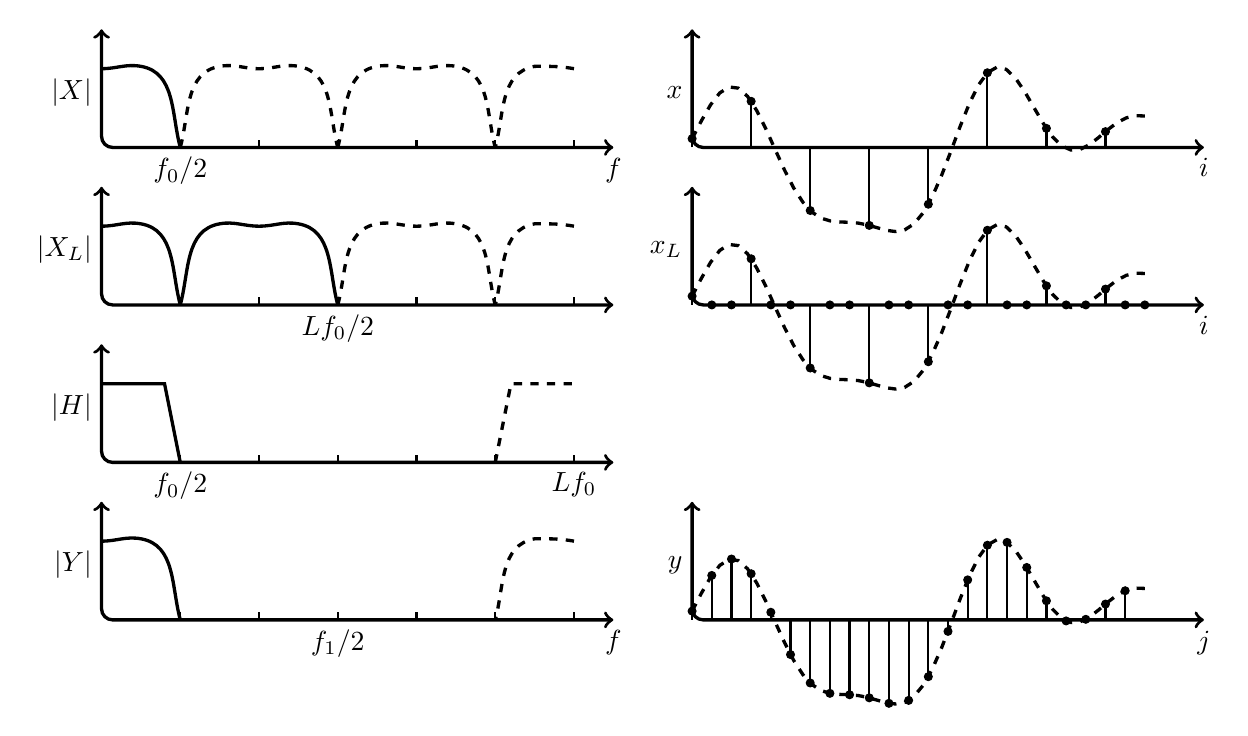
\begin{tikzpicture}[
declare function={ 
    funcx(\x) = -0.5*sin(2*pi*0.2*\x r) + 0.2*cos(2*pi*0.32*\x r) + 
                0.3*sin((2*pi*0.9*\x - 0.3) r) + 0.6*sin(2*pi*0.5*\x r);},
]
% frequency domain

%% |X|
\draw [<->, rounded corners, very thick](\falign,1.5) -- (\falign,0) --(\falign+6.5,0) node[below] {$f$};
\node[left] at (\falign,0.7) {$|X|$};
\node[below] at (\falign+1,0) {$f_0/2$};
\foreach \i in {1,...,6}
  \draw[thick] (\i, 0) -- (\i,0.1);
  \draw[very thick] (\falign,1) to [out=0, in=170] 
                    (0.5+\falign,1.03) to [out=350, in=105] 
                    (\falign+1,0);
  \draw[very thick,dashed] (\falign+1,0) to [out=75, in=190]  
                           (\falign+1.5,1.03) to [out=10, in=180] 
                           (\falign+2, 1) to [out=0,in=170] 
                            (\falign+2.5, 1.03) to [out=350, in=105] 
                            (\falign+3,0);
  \draw[very thick,dashed] (\falign+3,0) to [out=75, in=190]  
                            (\falign+3.5,1.03) to [out=10, in=180] 
                            (\falign+4, 1) to [out=0,in=170] 
                            (\falign+4.5, 1.03) to [out=350, in=105] 
                            (\falign+5,0);
  \draw[very thick,dashed] (\falign+6-0,1) to [out=170, in=0] 
                            (\falign+6-0.5,1.03) to [out=190, in=75] 
                            (\falign+6-1,0);

  %% W
  \draw [<->, rounded corners, very thick](\falign,-0.5) -- (\falign,-2) -- (\falign+6.5,-2);
  \node[left] at (\falign,0.7-2) {$|X_L|$};
  \node[below] at (\falign+3,-2) {$Lf_0/2$};
  \foreach \i in {1,...,6}
    \draw[thick] (\i, -2) -- (\i,0.1-2);
  \draw[very thick] (\falign,1-2) to [out=0, in=170] 
                    (0.5,1.03-2) to [out=350, in=105] 
                    (\falign+1,-2);
  \draw[very thick,] (\falign+1,-2) to [out=75, in=190]  
                     (\falign+1.5,1.03-2) to [out=10, in=180] 
                     (\falign+2, 1-2) to [out=0,in=170] 
                     (\falign+2.5, 1.03-2) to [out=350, in=105] 
                     (\falign+3,-2);
  \draw[very thick,dashed] (\falign+3,-2) to [out=75, in=190]  
                            (\falign+3.5,1.03-2) to [out=10, in=180] 
                            (\falign+4, 1-2) to [out=0,in=170] 
                            (\falign+4.5, 1.03-2) to [out=350, in=105] 
                            (\falign+5,-2);
  \draw[very thick,dashed] (\falign+6-0,1-2) to [out=170, in=0] 
                            (\falign+6-0.5,1.03-2) to [out=190, in=75] 
                            (\falign+6-1,-2);

%% H
  \draw [<->, rounded corners, very thick](\falign,-2.5) -- (\falign,-4) -- (\falign+6.5,-4);
  \foreach \i in {1,...,6}
    \draw[thick] (\i, -4) -- (\i,0.1-4);
  \node[left] at (\falign,0.7-4) {$|H|$};
  \node[below] at (\falign+1,-4) {$f_0/2$};
  \node[below] at (\falign+6,-4) {$Lf_0$};
  \draw[very thick] (\falign+0,1-4) -- (\falign+0.8,1-4) -- (\falign+1,0-4);
  \draw[very thick,dashed] (\falign+5,0-4) -- (\falign+5+0.2,1-4) -- (\falign+6,1-4);

  %% Y = H \ast X_L 
  \draw [<->, rounded corners, very thick](\falign,-4.5) -- (\falign,-6) -- (\falign+6.5,-6) node[below] {$f$};
  \foreach \i in {1,...,6}
    \draw[thick] (\i, -6) -- (\i,0.1-6);
  \node[left,align=right] at (\falign,0.7-6) {$|Y|$};
  \node[below] at (\falign+3,-6) {$f_1/2$};
  \draw[very thick] (\falign,1-6) to [out=0, in=170] 
                    (0.5,1.03-6) to [out=350, in=105] 
                    (\falign+1,-6);
  \draw[very thick,dashed] (\falign+6-0,1-6) to [out=170, in=0] 
                            (\falign+6-0.5,1.03-6) to [out=190, in=75] 
                            (\falign+6-1,-6);

  %%%%%%%%%%%%%%%
  % time domain
  %% x
  \draw [<->, rounded corners, very thick](\talign,1.5) -- (\talign,0) -- (\talign+6.5,0) node[below] {$i$};
  \node[left] at (\talign,0.7) {$x$};
  \foreach \i in {0,...,7}
    \draw[thick] (3*\i/4+\talign,0) -- (3*\i/4+\talign,{funcx(\i/2.)});
  \foreach \i in {0,...,7}
    \draw[fill] (3*\i/4+\talign,{funcx(\i/2.)}) circle[radius=0.05];
  \draw[very thick, dashed, domain=0:23,samples=50] plot(\x/4+\talign, {funcx(\x/6.)});

  %% x_L
  \draw [<->, rounded corners, very thick](\talign,-0.5) -- (\talign,-2) -- (\talign+6.5,-2) node[below] {$i$};
  \node[left] at (\talign,0.7-2) {$x_L$};
  \foreach \i in {0,...,7}{
    \draw[thick] (3*\i/4+\talign,-2) -- (3*\i/4+\talign,{funcx(\i/2.)-2});
    \draw[fill] (3*\i/4+\talign,{funcx(\i/2.)-2}) circle[radius=0.05];}
  \foreach \i in {0,...,7}
    \foreach \j in {1,2} 
    \draw[fill] (3*\i/4+\talign+\j/4,0-2) circle[radius=0.05];
  \draw[very thick, dashed, domain=0:23,samples=50] plot(\x/4+\talign, {funcx(\x/6.)-2});

 %% y
  \draw [<->, rounded corners, very thick](\talign,-4.5) -- (\talign,-6) -- (\talign+6.5,-6) node[below] {$j$};
  \node[left] at (\talign,0.7-6) {$y$};
  \foreach \i in {0,...,22}{
    \draw[thick] (\i/4+\talign,-6) -- (\i/4+\talign,{funcx(\i/6.)-6});
    \draw[fill] (\i/4+\talign,{funcx(\i/6.)-6}) circle[radius=0.05];}
  \draw[very thick, dashed, domain=0:23,samples=50] plot(\x/4+\talign, {funcx(\x/6.)-6});

\end{tikzpicture}
\caption{A sketch of upsampling when $L = 3$. The left column shows how the spectrum changes with each operation
and the right column mirrors the effect in the time domain.}
\label{fig:upsampling}
\end{figure}

\section{Sample Rate Conversion} \label{sec:src_basics}

Sample rate conversion, or resampling, is the process of taking a digital signal ($x[i]$) sampled at some rate 
($f_0$) and calculating new samples ($y[i]$) at a different rate ($f_1$).  To analyze this problem we use the 
ratio between the two rates: $f_1/f_0 = L/M$, where $L$ and $M$ are relatively prime integers.  A sample rate 
conversion can be helpfully thought of as the combination of upsampling and downsampling 
\citep{oppenheim10,lyons11}.  
Upsampling, (also commonly called interpolation or expansion), increases the sampling rate 
by a factor of $L$ with the insertion of $L-1$ zeroes between the original $x[i]$.  A low-pass, 
anti-imaging filter smooths the signal and supresses the high frequency spectral images greater than the original 
$f_0$ that have been introduced by the zero inserts.  Figure \ref{fig:upsampling} sketches this process in the 
time and frequency domain for when $L$ equals 3. 

 %% cartoon explaining down-sampling
 % http://tex.stackexchange.com/questions/124878/declare-function-for-tikzpicture
\begin{figure}[t!]
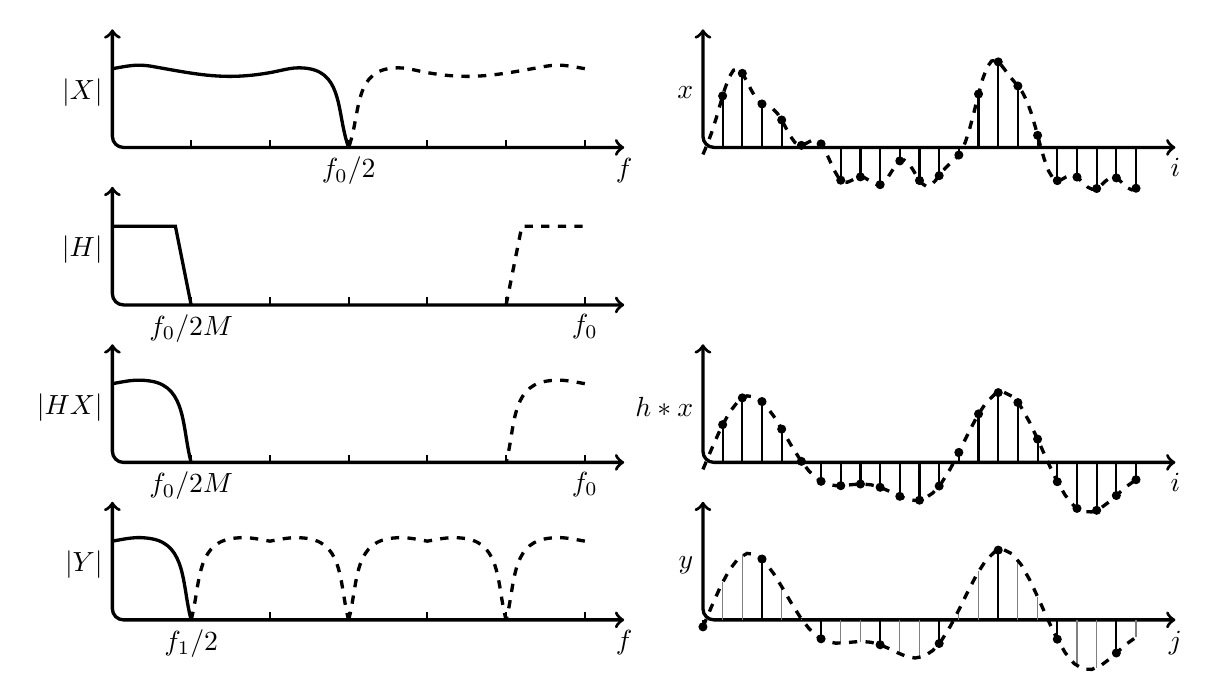
\begin{tikzpicture}[
declare function={ 
    funcx(\x) = -0.1*sin(2*pi*2.8*\x r) + 0.2*sin(2*pi*1.3*\x r) + 
                0.3*sin((2*pi*0.9*\x - 0.3) r) + 0.6*sin(2*pi*0.5*\x r);
    funchx(\x) = 0.3*sin((2*pi*0.9*\x - 0.3) r) + 0.6*sin(2*pi*0.5*\x r);},
]
  % frequency domain 

  %% |X(f)|
  \draw [<->, rounded corners, very thick](0,1.5) -- (0,0) --(6.5,0) node[below] {$f$};
  \node[left] at (0,0.7) {$|X|$};
  \foreach \i in {1,...,6}
    \draw[thick] (\i, 0) -- (\i,0.1);
  \node[below] at (3,0) {$f_0/2$};
  \draw[very thick] (0,1) to [out=10, in=170] (0.5,1.03)
                        to [out=350, in=190] (2,0.95) 
                        to [out=10, in=170] (2.5,1)
                        to [out=-10, in=110] (3,0);
  \draw[very thick,dashed] (6-0,1) to 
                            [out=170, in=10] (6-0.5,1.03) to 
                            [out=190, in=350] (6-2,0.95) to 
                            [out=170, in=10] (6-2.5,1) to [out=190, in=70] (6-3,0);

  %% |H(f)|
  \draw [<->, rounded corners, very thick](0,-0.5) -- (0,-2) -- (6.5,-2);
  \node[left] at (0,0.7-2) {$|H|$};
  \foreach \i in {1,...,6}
    \draw[thick] (\i, -2) -- (\i,0.1-2);
  \node[below] at (1,0-2) {$f_0/2M$}; \node[below] at (6,0-2) {$f_0$};
  \draw[very thick] (0,1-2) -- (0.8,1-2) -- (1,0-2);
  \draw[very thick,dashed] (5,0-2) -- (5.2,1-2) -- (6,1-2);

  %% |W(f)|
  \draw [<->, rounded corners, very thick](0,-2.5) -- (0,-4) -- (6.5,-4);
  \node[left] at (0,0.7-4) {$|HX|$};
  \foreach \i in {1,...,6}
    \draw[thick] (\i, -4) -- (\i,0.1-4);
  \node[below] at (1,0-4) {$f_0/2M$}; \node[below] at (6,0-4) {$f_0$};
  \draw[very thick] (0,1-4) to [out=10, in=170] (0.5,1.03-4) to [out=350, in=105] (1,0-4);
  \draw[very thick,dashed] (6-0,1-4) to [out=170, in=10] (6-0.5,1.03-4) to [out=190, in=75] (6-1,0-4);

  %% Y(f)
  \draw [<->, rounded corners, very thick](0,-4.5) -- (0,-6) -- (6.5,-6) node[below] {$f$};
  \node[left] at (0,0.7-6) {$|Y|$};
  \foreach \i in {1,...,6}
    \draw[thick] (\i, -6) -- (\i,0.1-6);
  \node[below] at (1,0-6) {$f_1/2$}; 
  \draw[very thick] (0,1-6) to [out=10, in=170] (0.5,1.03-6) to [out=350, in=105] (1,0-6);
  \draw[very thick,dashed] (1,0-6) to [out=75, in=190]  (1.5,1.03-6) to [out=10, in=170] 
                            (2, 1-6) to [out=10,in=170] (2.5, 1.03-6) to [out=350, in=105] (3,-6);
  \draw[very thick,dashed] (3,0-6) to [out=75, in=190]  (3.5,1.03-6) to [out=10, in=170] 
                            (4, 1-6) to [out=10,in=170] (4.5, 1.03-6) to [out=350, in=105] (5,-6);
  \draw[very thick,dashed] (6-0,1-6) to [out=170, in=10] (6-0.5,1.03-6) to [out=190, in=75] (6-1,0-6);

  %%%%%%%%%%%%%%%
  % time domain
  %% x
  \draw [<->, rounded corners, very thick](7.5,1.5) -- (7.5,0) -- (13.5,0) node[below] {$i$};
  \node[left] at (7.5,0.7) {$x$};
  \foreach \i in {1,...,22}{
    \draw[thick] (\i/4+7.5,0) -- (\i/4+7.5,{funcx(\i/6.)});
    \draw[fill] (\i/4+\talign,{funcx(\i/6.)}) circle[radius=0.05];}
  \draw[very thick, dashed, domain=0:22,samples=100] plot(\x/4+7.5, {funcx(\x/6.)});

  %% h \ast x
  \draw [<->, rounded corners, very thick](7.5,1.5-4) -- (7.5,0-4) -- (13.5,0-4) node[below] {$i$};
  \node[left] at (7.5,0.7-4) {$h\ast x$};
  \foreach \i in {1,...,22}{
    \draw[thick] (\i/4+7.5,-4) -- (\i/4+7.5,{funchx(\i/6.)-4});
    \draw[fill] (\i/4+\talign,{funchx(\i/6.)-4}) circle[radius=0.05];}
  \draw[very thick, dashed, domain=0:22,samples=50] plot(\x/4+7.5, {funchx(\x/6.)-4});

  %% y 
  \draw [<->, rounded corners, very thick](7.5,1.5-6) -- (7.5,0-6) -- (13.5,0-6) node[below] {$j$};
  \node[left] at (7.5,0.7-6) {$y$};
  \foreach \i in {1,...,22}
    \draw[gray] (\i/4+7.5,-6) -- (\i/4+7.5,{funchx(\i/6.)-6});
  \foreach \i in {0,...,7}{
    \draw[thick] (3*\i/4+7.5,-6) -- (3*\i/4+7.5,{funchx(3*\i/6.)-6});
    \draw[fill] (3*\i/4+\talign,{funchx(3*\i/6.)-6}) circle[radius=0.05];}
  \draw[very thick, dashed, domain=0:22,samples=50] plot(\x/4+7.5, {funchx(\x/6.)-6});


\end{tikzpicture}
%\caption{Series of steps for down sampling shown in the frequency domain when $M=3$.}
\caption{A sketch of downsampling when $M = 3$. The left column shows how the spectrum changes with each operation
and the right column mirrors the effect in the time domain.}
\label{fig:downsampling}
\end{figure}

Downsampling, or decimation, by an integer factor of $M$ requires that the signal be first low-pass filtered to 
avoid aliasing at frequencies greater than the desired rate $f_0/M$.  Next, the sampling rate is reduced to 
$f_0/M$ by selecting every $M$th sample from the filtered signal.  Figure \ref{fig:downsampling} shows this 
process in the time and frequency domain for when $M$ equals 3.

Sample rate conversion by a factor $L/M$ can be conceptualized as a three step process where the original signal 
is expanded by $L$, filtered, and then decimated by $M$.  As illustrated by Figure \ref{fig:resample_basic}, 
the serial anti-imaging and 
anti-aliasing filters are combined into a single filter with cutoff frequency of 
$1/\mathrm{max}(L,M) \times Lf_0/2$.  Under this scheme, interpolation must precede decimation otherwise desired 
frequency components greater than $f_0/M$ cannot be preserved.

Computationally, this basic sample rate conversion scheme is highly inefficient.  The filtering is applied at 
the highest possible sample rate, $Lf_0$, on a time-series that is $(L-1)/L$ zeros by fraction. Furthermore, the 
decimator discards an $(M-1)/M$ fraction of the samples.  As a result, this algorithm requires a lot of memory 
and spends precious clock time with wasted math.  There is a vast literature of techniques and algorithms that 
improve performance including multistage resampling, folded filter structures, and polyphase representations 
\citep{oppenheim10,lyons11,vaidyanathan93}.

\begin{figure}[t]
\centering
\begin{tikzpicture}
   \node[dspnodeopen,dsp/label=left]  (c0) {$x[i]$};
   \node[dspsquare,right=of c0]                     (c1) {\upsamplertext{L}};
   \node[dspfilter,right=of c1]                     (c2) {$H(\z)$};
   \node[dspsquare,right=of c2]                    (c3) {\downsamplertext{M}};
   \node[dspnodeopen,right=of c3,dsp/label=right]  (c4) {$y[j]$};
   \foreach \i [evaluate = \i as \j using int(\i+1)] in {0,1,...,3}
       \draw[dspconn] (c\i) -- (c\j);
\end{tikzpicture}
\caption{Basic multirate resampling signal flow graph.}
\label{fig:resample_basic}
\end{figure}

There have been recent development of polyphase filter representations for GPUs
\citep[i.e.][]{vanderveldt12,adamek14,kim14a}.  These filter structures can operate at the low sample rate of 
$f_0/M$
by introducing delays to switch the expander and decimatator \citep{crochiere81}.  However, they require 
some filter design and careful book-keeping or buffering to keep track of sample indices \citep{wang01}.
The implementation in \citet{kim14a} assigned each thread to a filter coefficient, parallelizing the 
inner product operation.  However, \citet{kim14a} found that their GPU kernel was dominated by the 
indexing operations.  \citet{adamek14} (building on the work by \citet{vanderveldt12}) presented an
implementation of a polyphase filter bank that could run at data rates in excess of 6.5\,GB/s 
(their estimate for the single channel output of the SKA's Low Frequency Aperture Array).

%  https://github.com/wesarmour/astro-accelerate
\begin{figure}[t!]
\epsscale{1.0}
\plotone{aphids/windows.eps}
\caption{Frequency response for FIR filters equivalent to linear and nearest interpolation when $L/M = 64/39$.
The orange region shows the first Nyquist zone of the target $L/Mf_0$ sample rate.  Spectral components at all 
other frequencies are aliased into this region.}
\label{fig:windows}
\end{figure}

For testing and development we also considered two elementary options for the resampling: linear and nearest 
neighbor interpolation.  Linear interpolation is:
\begin{equation}
y[i] = x[j] + (x[j+1] - x[j]) (if_0/f_1 - j)
\end{equation}
where $j = \mathrm{floor}(if_0/f_1)$.  This is equivalent to applying a ``tent'' FIR filter with $2L$ taps on the 
upsampled $Lf_0$ time series before decimation \citep{oppenheim10}.  Similarly, a $2L$ tap box-car filter is 
equivalent to nearest-neighbor interpolation:
\begin{equation}
y[i] = x[\mathrm{round}(if_0/f_1)].
\end{equation}

Neither linear or nearest-neighbor interpolation consider the frequency content of the original signal and, as a 
result, perform poorly for signals with any significant power near the Nyquist rate \citep{fraser89}.  To further 
emphasize this point, Figure 
\ref{fig:windows} shows the frequency response for both methods when 
the resampling factor $L/M$ is $64/39$.  Note that both methods have large side lobes and so the 
resampled signal will introduce a large slope in the passband.  However, GPUs can compute 
these low-order interpolations directly on the card using texture memory.  \citet{kim14b} utilize this feature 
by using the cuFFT library to upsample the signal in the Fourier domain by some initial factor, $U$, and then 
interpolating in texture memory.  It would be straight forward to 
expand upon the framework introduced by \citet{kim14b} to handle cases where $M$ is greater than $L$.  
This scheme should help reduce loss from aliasing, albeit 
at the cost of two FFTs and much larger memory requirements.

 
\subsection{Resampling in the Fourier Domain} \label{sec:fourier_resampling}
In contrast to the previous methods, one can also implement a rational $L/M$ sample rate conversion entirely in 
the Fourier domain \citep{gold69}.  After accumulating $kM$ samples at a clock rate of $f_0$ 
(where $k=1,2,3\ldots$), the DFT 
returns spectral components spaced at $f_0/kM$.  If $f_1 > f_0$, the resampled spectrum is generated by inserting
$p$ zeros to match the new $f_1$ while maintaining the correct frequency components: 
\begin{equation}
\frac{f_1}{kM+p} = \frac{f_0}{kM}.
\end{equation} 
Solving for $p = k(L - M)$.  If $f_0 < f_1$, the spectrum is instead trimmed by $p$ samples.  The time series
sampled at $f_1$ can then be constructed from the inverse DFT.  This method is equivalent to sinc 
interpolation using an ideal low-pass filter and is a perfect interpolator
if the original, continuous signal has a discrete spectral density distribution that is band-limited below the 
Nyquist limit.  In practice, errors may be introduced from aliased spectral leakage. 

Trimming or padding the spectrum is equivalent to convolving a normalized sinc function with the original series 
wrapped periodically.  Consequenty, errors will be introduced into the beginning and end of the
resampled signal.  How far and significantly this error propagates away from the time series' edges depends 
on the width of the sinc function which is set by the resampling factors $L$ and $M$: 
\begin{equation} \label{eq:sinc}
B\,\mathrm{sinc}(B t) \overset{\mathcal{F}}{\Longleftrightarrow} \begin{cases} 1 \quad |f| < B/2 \\ 0 \quad |f| > B/2 \end{cases}
\end{equation}
where $B = \mathrm{min}(f_0,L/Mf_0)$.  
The number of samples for which this makes a large difference is small and can be roughly treated as less than a 
1\% effect when $N > 100\,\mathrm{max}(L/M,1)$.  One option to mitigate this error to stitch together 
overlapping, resampled segments \citep{bi11} which requires more computation and memory.  A second strategy is to 
multiply the original signal by some tapered window function \citep{fraser89}.

For post-processing phased SWARM, DFT resampling is a good fit because one can access large chunks of 
the time series without accumulators in hardware and it has well-behaved errors
that can be easily modeled.  However, the speed of the FFT depends on the resampling factors ($L/M = 32/39$ for 
the March 2015 EHT observations) and zero-padding in the case that the $L\gg M$ may require large amounts of 
memory.  In practice, we also found that the memory space of the GPU could be a limiting factor not only 
on how much data could be simultaneously resampled, but also storing FFT plans (which depends on
values of $L$ and $M$).

%% Loss table : /home/krosenfe/resampling/losses.py
% losses for FIR filtering, interpolation schemes, and FFT
\begin{table}
\begin{center}
\centering
\caption{Correlation coefficient loss from resampling \label{tab:loss}}
\begin{threeparttable}
\begin{tabular}{l|ccc}
\toprule
Method & 64/39 & 32/39 & 128/125 \\
\midrule
Nearest-Neighbor            & 13\% & 17\% & 13\% \\
Linear                      &  5\% &  7\% &  5\% \\
Hamming window ($16L$ taps) &  1\% &  2\% &  2\% \\
FFT ($N=M$)                 &  1\% &  1\% & 0.2\% \\
\bottomrule
\end{tabular}
\end{threeparttable}
\end{center}
\end{table}

\tikzstyle{line} = [draw,-latex']
\tikzstyle{cpu} = [rectangle, draw, fill=blue!20,
    text width=5em, text centered, rounded corners, minimum height=4em]
\tikzstyle{gpu} = [rectangle, draw, fill=red!20,
    text width=5em, text centered, rounded corners, minimum height=4em]
\tikzstyle{resamp} = [rectangle, draw, minimum height=4.5em, align=center, minimum width=15em] 

\begin{figure}[t!]
\linespread{1.}\selectfont{}
\begin{center}
\begin{tikzpicture} [node distance = 5cm, auto]
\node [cpu] (mark6_in) {Mark6 Reader};
\node[gpu,below of=mark6_in](reader){Reader};
\node[gpu,right of=reader](resampler){Resampler};
\node[cpu,right of=resampler](VDIF_pkt){VDIF packet \\ \& header};
\node[cpu,below of=VDIF_pkt](mark6_out){Mark6 Writer};

\path[line] (mark6_in) -- node[align=center] {BENG @ 2496 GHz \\ quantized to 2-bits}(reader);
\path[line] (reader) -- node[align=center] {spectra of \\ 16k complex64} (resampler);
\path[line] (resampler) --  node[align=center] {time series \\ @ 2048 GHz}(VDIF_pkt);
\path[line] (VDIF_pkt) -- node[align=center, left]{VDIF @ 4096 GHz \\ quantized to 2-bits}(mark6_out);
\end{tikzpicture}
\caption{This signal flow chart shows an overview of APHIDS.  The red boxes represent operations on the GPU 
while blue boxes are for the CPU.  Once the B-engine frames have been unpacked, each of the two phased sum 
streams are processed independently and in a serial fashion.}
\label{fig:aphids_flow_chart}
\end{center}
\end{figure}

\section{APHIDS} \label{sec:aphids}

We are developing a software solution to the resampling problem called APHIDS.  This 
open-source project is written in C/CUDA using
the High Availibility Shared Pipeline 
(HASHPIPE)\footnote{\url{https://github.com/david-macmahon/hashpipe}}.  The software is designed to use 
modularized, lightweight threads to handle reading data packets from hard drives, resampling on a GPU cluster, 
and then writing back to separate disks.  These three steps are each loosely mapped to threads we call the 
vdif\_in\_net thread, vdif\_inout\_gpu\_thread, and vdif\_out\_net thread. 
The ultimate goal of is to process data streamed directly at the telescope.  The flowchart in Figure 
\ref{fig:aphids_flow_chart} shows how data progresses 
through the pipeline and this section will describe each block covering the major hardware components, software 
design, and data formats.  We will conclude with a discussion of future development and applications of APHIDS.


\subsection{Hardware and Data description}

APHIDS features three main hardware components: an I/O data system, CPU, and GPU cluster.  For I/O, the 
EHT observations taken by SWARM in March 2015 have been stored on four disk-packs that each hold eight, 
6\,TB hard drives (totaling 192\,TB of disk space).  The Mark6 VLBI data system has four modules 
that can hold one disk-pack and we use
two seprate Mark6 units to handle the recording and playback of data.  APHIDS itself is run on a separate CPU 
that controls the GPU cluster.

The GPU cluster has four GTX 980 GPUs, each with 4GB of local memory.  Data from the CPU (or host) is copied over 
a PCI-E bus into the local GPU (or device) memory.  Once the data is transferred, the host directs the device
to perform functions (or kernels) on the data which must be again moved from the local device memory onto 
on-chip memory for the individual streaming multiprocessors that make up the GPU.  After computation is done, 
the host transfers the data off of the device memory.

The observations were recorded using a scatter/gather file system which disperses the 
individual scan data over the four modules in a Mark6.  APHIDS uses fast, general purpose software called 
sgcomm (Scatter/Gather Communication) to read in 
the scattered data into CPU shared memory over a 10 Gigabit Ethernet.  Data from phased SWARM was 
streamed through a specialized version of the R2DBE called the SDBE (Swarm Digital Back End) and packaged into
a customized B-engine format.  Each B-engine frame is composed of 2048, 1056B VDIF frames 
\footnote{\url{http://www.vlbi.org/vdif/}} with 128 snapshots of a 
16384 sample SWARM spectra.  However, the current SDBE bitcode packs
neither the snapshots contiguously in time nor the spectrum samples contiguously in frequency.  Furthermore, 
each B-frames overlaps the preceding one in memory.  Our resampling algorithm handles $19968$\,SWARM samples
simultaneously, so in order to reduce the amount of book-keeping the inout thread buffers 40 B-engine frames to 
produce $39 \times 128$ complete SWARM snapshots.  The inout thread does preliminary checks to ensure that the 
B-engine frames are complete before assigning each buffer to a GPU.  The data is written as a time series using 
following the VDIF specification.

As mentioned previously, the data is split into two phased sums that together cover the desired 4096\,MHz of 
observing bandwidth.  Since DIFX can handle the chunks independently we do not stitch the spectra together. 
However, the observation was designed to include guard bands which must be removed by APHIDS 
(see Figure \ref{fig:swarm_amp_spec} and \S\ref{sec:resamp_block}).

\begin{figure}[t!]
\linespread{1.}\selectfont{}
\centering
\begin{tikzpicture}[node distance = 2.2cm, auto]
\node[align=center](init){};
\node[resamp,below of=init](irfft){(A) batched real IFFT \\ dimension of $32768$};
\node[resamp,below of=irfft](rfft){(B) batched real FFT \\ dimension of $39 \times 512$};
\node[resamp,below of=rfft](trim){Trim band and shift frequency};
\node[resamp,below of=trim](rifft){(C) batched real IFFT \\ dimension of $32 \times 512$};
\node[align=center,below of=rifft](final){};

\path[line](init) -- node[align=left]{ complex spectra \\ @ 2496\,MHz} (irfft);
\path[line](irfft) -- (rfft);
\path[line](rfft) -- (trim);
\path[line](trim) -- (rifft);
\path[line](rifft) -- node[align=left]{ time series \\ @ 2048\,MHz}(final);
\end{tikzpicture}
\caption{The resampling block trims the phased SWARM guard bands and shifts the passband to DC as part of the 
resampling operation.}
\label{fig:resampling_block}
\end{figure}


\subsection{Resampling Block}\label{sec:resamp_block}

APHIDS resamples the data in the Fourier domain (see \S \ref{sec:fourier_resampling}).  There were several 
contributing factors that led us to make
this choice rather than apply filters in the time domain.  First, the GPU cluster can handle relatively large 
chunks of data at a time so losses from the DFT are very manageable.  Second, regardless of 
what resampling algorithm is used the SWARM spectra must 
be transformed into the time domain, the guard bands trimmed and the signal modulated.  These operations are done 
naturally in the Fourier domain.  However, the cost of the resampling operation will be largely dominated by 
these operations.  Lastly, we can utilize the optimized cuFFT library
\footnote{\url{https://developer.nvidia.com/cuFFT}} to ensure good performace, reduce development time and 
maintain a manageably sized codebase.

The APHIDS resampling block is composed of three 1-dimensional FFTs (A, B, and C; see Figure 
\ref{fig:resampling_block}).  Following the cuFFT API reference to improve performace, we utilize batched
FFTs (launching more than one FFT at a time using the cuFFT API), out-of-place transforms, 
and operate on contiguous chunks of memory.  We also use single precision transforms to 
reduce the memory transfer bandwidth and ensure that 
the resampling block can be run on a single device.  The latter point is important since it allows the inout
thread to parallelize the resampling operation across the cluster and provide a roughly x4 speedup.


The first FFT (A) takes the complex valued, 16384 sample SWARM spectrum into the time domain, returning 
32768 real samples.  Since SWARM omits the Nyquist sample which is outside the SWARM guard band cutoff frequency, 
we insert a zero as the 16385th sample.  Since this transform is radix-2, the performance should benefit from 
the Cooley-Tukey algorithm.  However, on our cluster the cuFFT library exhibits linear improvement in Gflops 
with transform size up to N of 16384 (see Figure \ref{fig:C2R_performance}).  This behavior is consistent with 
the CUDA 7.0 performance 
report\footnote{\url{http://on-demand.gputechconf.com/gtc/2015/webinar/gtc-express-cuda7-performance-overview.pdf}} 
and we find that this transform, just ouside of the optimal regime, operates at 6.7 Gsps.

\begin{figure}[t!]
\epsscale{0.95}
\plotone{aphids/C2R_performance.eps}
\caption{This figure shows the performance of radix-2, single precision, batched, complex-to-real, 1D transforms 
measured on our GPU cluster (solid lines). The dashed lines show the same measures for non radix-2, candidate 
resampling FFT sizes ($N_B$).  The benchmark conventions follow FFTW  (http://www.fftw.org/speed/method.html).}
\label{fig:C2R_performance}
\end{figure}

Next, we Fourier transform chunks of $N_B = 19968$ consecutive time series samples (B).  The resulting 
spectrum has a frequency resolution of $2496$\,MHz$/19958=125$\,kHz.  The folllowing step is to apply a third
complex-to-real transform (C) on a subset of the spectrum, using only frequences from $150$\,MHz to $1174$\,MHz.  
The final time series has size $N_C= 2\times(1174-150)/0.125=16384$ per batch element and our desired 
sampling rate of 
$16384 \times 0.125$\,MHz$ = 2048$\,MHz.  This simple operation simultaneously resamples the signal, modulates 
the signal, and trims the guard bands.  Furthermore, it is easily implemented using cuFFT by using the same 
batch size as the second real-to-complex transform, increasing the input pointer index by $150 / 0.125 = 1200$
(equivalent to masking out the first 1200 channels) and then using a input stride of $9980$ for the 
$N=16384$ complex-to-real transform.

The choice of FFT size was set to maximize performance.  In order for the target sampling rate to be achieved
$N_B$ must be a multiple of 39.  Furthermore, so that the 150\,MHz guard band can be removed, we must ensure that 
150 is a multiple of $2496/N_B$:
\begin{equation}
\frac{150\times39}{2496} = \frac{75}{32} = \frac{i}{j}, \quad i,j = 1, 2,3, \ldots
\end{equation}
To ensure this, $j$ should be a multiple of 32 so that 
\begin{equation}
N_B = 39j = 1248i, \quad i=1,2,3,\ldots
\end{equation}
Lastly, the size of the C transform is then determined:
\begin{equation}
N_C = \frac{32}{39} N_B.
\end{equation}
The dashed line in Figure \ref{fig:C2R_performance} shows the performance for candidate $N_B$s.  Unlike for 
the radix-2 cases, the configuration that has the best Gflop performance does not also provide the best Gsps
rate.  This is likely because the Gflop calculation is not an actual flop count, but a scaling from the 
original Cooley-Tukey algorithm \citep{cooley65}.  The Gsps metric is perhaps more useful in this case as it
shows that choices of $N_B \leq 19968$ will have good performance.  However, the figure also demonstrates
that this non radix-2 FFT is about $2\times$ slower than the radix-2 case.

\subsection{Timing Performance}

In this section we report on timing measurements of the APHIDS resampling kernels.  We consider the cost of 
loading the data onto the device separately and do not include it in the scores of the individual kernels.  
Furthermore, we do not include the cost of building the FFT plan since this operation is done only once.
We have designed the resampling block to operate on a single GPU so there is no time spent moving data 
between devices and we can parallelize across each card.  The
kernels (except for the depacketer) must be called
twice, once on each phased sum.  Our current implementation uses synchronous calls (one kernel function is 
called at a time).  We tested an asynchronous setup, but saw no speedup.  This indicates that the majority of 
the GPU resources are being used.  Table \ref{tab:kernel_times} lists the time it takes for the kernel to be 
executed a single time and also the speed of the kernel assuming it is operating on a buffered 0.32\,Gb data 
chunk (see \S\ref{sec:resamp_block}).

%% Loss table : /home/krosenfe/resampling/losses.py
% losses for FIR filtering, interpolation schemes, and FFT
\begin{table}
\begin{center}
\caption{Timing measurements of APHIDS kernels \label{tab:kernel_times}}
\begin{threeparttable}
\begin{tabular}{l|cc}
\toprule
Kernel & time [ms] & rate [Gbps] \\
\midrule
Reorder                & 10.5 & 31.5 \\
FFT A (N=32768)        & 25.4 & 12.9 \\
FFT B (N=19968)        & 38.0 & 8.6  \\
FFT C (N=16384)        & 13.8 & 23.7 \\
Quantize (2-bit)       & 12.0 & 27.3 \\
\bottomrule
\end{tabular}
\end{threeparttable}
\end{center}
\end{table}

\subsection{FFT Accuracy}
One concern with using multiple FFTs to change the sampling rate is the error introduced by bit growth.  The 
floating point error grows as $\mathcal{O}(\sqrt{\log{N}})$ \citep{schatzman96} on average for the Cooley-Tukey
algorithm, but errors can be exacerbated by innacurate twiddle factors or our choice of FFT algorithm (see
benchFFT\footnote{\url{http://www.fftw.org/accuracy/}}).  We have computed the accuracy of the cuFFT library 
using single precision for 
radix-2 transforms as well as the $N_b = 19968$ case in Figure \ref{fig:fft_accuracy}.  These values 
were computed using benchFFT and we compare against fftw3\footnote{\url{http://www.fftw.org/}}
results also computed on our GPU cluster.  For random input, the cuFFT library follows the expected 
$\mathcal{O}(\sqrt{\log{N}})$ behavior, but with larger scatter and slightly worse performance than fftw3.

\begin{figure}[t]
\plotone{aphids/fft_accuracy.eps}
\caption{Accuracy of the FFT algorithm as measured by the $L_2$ error from benchFFT} \label{fig:fft_accuracy}
%/home/krosenfe/testing/cufft_accuracy/make_figure.py
\end{figure}

Round off error and bit growth is also a general concern for scientific computing on GPUs.  
Increasing the precision to double can significantly slow down performance and then 
require reoptimization or even the redesign of kernels.  Generally, well implemented FFTs can 
be very stable options.  The results of ours test suggest that 
bit growth will not be a large source of loss for the resampling scheme presented in \S\ref{sec:resamp_block}.

\subsection{Quantization}
Another source of loss and distortion to consider is the requantization back to 2-bits that is done
before writing back to disk on the Mark6 (see Figure \ref{fig:aphids_flow_chart}).  In theory, APHIDS could 
record higher bit data (or even the full 32 bits for floating point), but this adds complications for 
correlation 
in DIFX and would incur costs for both disk space and output data rate.  While the former cost is monetary, the 
latter could be an important limiting factor for real-time operation of APHIDS at the back end of the SDBE.  
The signal-to-noise loss expected from 2-bit quantization is a function of the quantization 
thresholds, but for Gaussian noise and Nyquist sampling is at best 12\% \citep{cooper70,thompson01}.

\subsection{Inverting the Polyphase Filterbank}
Under normal operation, SWARM uses a polyphase filter bank (PFB) to generate its spectra.  The PFB is an 
efficient method of producing spectra where each channel has a frequency response much better than the 
sinc pattern of the DFT.  This is achieved by using a window function and a polyphase filter structure to reduce 
the effects of leakage and scalloping \citep{lyons11}.  However, for VLBI observations we must transform the 
spectrum into the original time series to resample the data.  Inverting the PFB is a non-trivial operation so 
the operators use a version of the SWARM bit-code that replaces the PFB with an FFT.  However, for the first 
two nights of the 2015 EHT campaign this version was not used and so we must consider this problem.

One option is to simply apply the generic APHIDS pipeline on the PFB spectra which uses an DFT to invert the 
SWARM spectra into time series.  The resulting pseudo time-series is a series of weighted 
averages of the original time series.  The weights are determined by the window function used in the 
PFB and the number of elements in the sum by the number of taps, $N_T$.  For example, if the window function is 
a box car, then the weights are equal and the correlation coefficient for a white noise time stream goes like:
\begin{equation}
\rho = \frac{1}{\sqrt{N_T}}.
\end{equation}
SWARM uses four taps and a Hanning filter.  We simulated the resulting correlation loss and saw a 34\% loss, 
exceeding the largest loss we expect in the pipeline from the 2-bit quantization (12\%).  Using the PFB inversion
technique developed by Richard Shaw\footnote{\url{https://github.com/jrs65/pfb-inverse}} we see excellent 
recovery with a loss of only 0.5\% although the inversion routine takes about 10 times longer than numpy's
iFFT and already uses the highly optimized LAPACK library.  CUDA libraries offer many of the required functions 
to implement this solution on the GPU and we have ported Shaw's solution to CUDA using a combination of 
CUBLAS and CUSolver.  The current implementation runs about 5 times slower than an inverse FFT batched over 
the same size data chunk.

\begin{figure}[t!]
\epsscale{1.0}
\includegraphics{aphids/kr_autos.eps}
\caption{This figure shows the spectral density of phased SWARM along with the single reference dish 
(in purple).  The APHIDS output is also plotted (dotted).}
\label{fig:swarm_amp_spec}
\end{figure}

\subsection{Current Status and Future Development}

APHIDS is still under active development, but rapidly nearing full-scale production.  Figure \ref{fig:swarm_amp_spec}
shows the original SDBE and resampled auto spectra from data taken in March 2015.  Using data resampled by APHIDS, Mike Titus, 
the correlator engineer at MIT Haystack, has found a cosmic fringe on 3C297 using the short 
baseline between the JCMT and the SMA (see Figure \ref{fig:aphids_fringe}).  He reported an increase in the fringe amplitude over initial tests
using linear interpolation.  APHIDS currently runs about 4.5 times slower than real time, sufficient for 
processing the March 2015 EHT campaign data.  The resampling block with PFB inversion should be available
shortly.

APHIDS promises to be an important tool for the EHT.  It crucially enables the correlation in
DIFX of non-standard sampling rates and also provides a platform for any general pre-processing of 
VLBI data.  It features fast data I/O from Mark6 recorders and GPU accelarated processing.  
We have demonstrated the correctness and speed of this design and its immediate applicability to 
the 2015 EHT data.  However,
there remain a number of challenges for future development of the software.

For future VLBI campaigns at the SMA, it would be ideal if APHIDS could run in real-time 
at the backend of the SDBE.  This would reduce the media requirements and also the 
hassle of post-processing the data offsite.  However, the performance will need to improve as the
SWARM data rates increase and if the front-end of the pipeline is optimized to reduce the 
amount of SNR loss from quantization.  Additionally, some analysis on the cooling requiremeents 
of the cards should be conducted to ensure that the GTX980s used in our GPU cluster can safely run 
at the altitude of the SMA (4100\,meters).  Regardless of where it operates, APHIDS will need 
maintence to remain compatible with SWARM as it and the SDBE are updated.  The current 
git repository and its wiki is a good solution for keeping track of versioning and performance status.

%\includepdf[pages={1}]{aphids/089-0810_JS_fix.pdf}
\begin{figure}
\includegraphics[width=\linewidth]{aphids/089-0810_JS_fix.pdf}
\caption{Fourfit plots of a sky fringe found using APHIDS resampled SWARM data and JCMT.}
\label{fig:aphids_fringe}
\end{figure}

\section{The APHIDS Team}
Andre Young, Lindy Blackburn, Laura Vertatschitsch, Rurik Primiani, and Katherine Rosenfeld are part of 
the core APHIDS team located at the Smithsonian Astrophysical Observatory.  Jonathan Weintroub and Sheperd
Doeleman were responsible for project oversight and invaluable support was provided by Mike Titus and Geoff Crew at MIT
Haystack.  The EHT is supported by the NSF and the Gordon and Betty Moore Foundation.
